%%%%%%%%%%%%%%%%%%%%%%%%%%%%%%%%%%%%%%%%%
% Simple Sectioned Essay Template
% LaTeX Template
%
% This template has been downloaded from:
% http://www.latextemplates.com
%
%%%%%%%%%%%%%%%%%%%%%%%%%%%%%%%%%%%%%%%%%

%----------------------------------------------------------------------------------------
%	PACKAGES AND OTHER DOCUMENT CONFIGURATIONS
%----------------------------------------------------------------------------------------

\documentclass[12pt]{article} % Default font size is 12pt, it can be changed here

\usepackage{geometry} % Required to change the page size to A4
\geometry{a4paper} % Set the page size to be A4 as opposed to the default US Letter
\usepackage{amsmath}

\usepackage{graphicx} % Required for including pictures

\usepackage{float} % Allows putting an [H] in \begin{figure} to specify the exact location of the figure
\usepackage{lastpage}
\usepackage{fancyhdr}
\usepackage{url}
\usepackage{amsmath}



%Code packages

\usepackage[utf8]{inputenc}
\usepackage{listings}
\usepackage{color}
% Code packages end


\linespread{1.1} % Line spacing


\begin{document}

%----------------------------------------------------------------------------------------
%	TITLE PAGE
%----------------------------------------------------------------------------------------

\begin{titlepage}

\center % Center everything on the page

{\huge \bfseries Chaotic Scattering for a Sliding Mass in a Complex Topography}\\[0.4cm] % Title of your document

\textsc{\large Avi Vajpeyi}\\[0.5cm] % Major heading such as course name
\textsc{\large CS 200}\\[0.5cm]

{\large \today}\\[3cm]

\begin{abstract}
The Gaspard-Rice scattering model has been instrumental in framing the understanding of a wide range of chaotic scattering behavior problems in physical situations \cite{GRice}. This paper draws inspiration from the model to simulate chaotic scattering of a point particle that is released with four hills in its path. The simulation resembles most classical scattering systems with one impact parameter that causes the particle to scatter. The trajectories of the impact parameters are generated by numerically integrating differential equations of motion using various algorithms such as the Euler-Cromer and Runge-Kutta methods. While traversing across the hills, certain impact parameters lead to the particle getting trapped for a period inside the system before exiting at an angle measured from the horizontal axis. The angle of exit from the system is compared to the impact parameter, and is found to display chaotic nature at certain regions. Additionally, it is found that the correlation between the parameters demonstrates fractal behavior.
\end{abstract}

\vfill % Fill the rest of the page with whitespace
\end{titlepage}

\pagestyle{fancy}
\renewcommand{\headrulewidth}{0pt}
%\fancyhead[L]{Team \#YOUR NUMBER}
\setcounter{page}{2}
\fancyhead[R]{ Page \thepage\ of \pageref{LastPage}}
\fancyfoot{}

%----------------------------------------------------------------------------------------
%	TABLE OF CONTENTS
%----------------------------------------------------------------------------------------

\listoffigures
\tableofcontents % Include a table of contents

\newpage

%----------------------------------------------------------------------------------------
%	INTRODUCTION
%----------------------------------------------------------------------------------------

\section{Introduction} \label{Introduction}
Nature is extraordinarily intricate and unpredictable. In 1961, Edward Lorenz, a meteorologist, created a computer simulation to model weather \cite{WeatherSimulation}. He rounded an input parameter to three decimal places instead of the conventional six and was surprised to find the impact that this tiny alteration had on his long term forecasting abilities \cite{WeatherSimulation}. This highlighted the fact that small uncertainties can yield drastically different outcomes. Hence predicting the patterns of complicated systems such as the migratory pattern of birds, pandemics, or even patterns of the human heart, is nearly impossible, as these predictions require very high precision measurements. This gives rise to chaos theory, a discipline of mathematics that studies the behavior and conditions of sensitive systems \cite{chaoticIntro}. This paper examines chaotic scattering within chaos theory, a topic with applications in a wide range of fields including nuclear physics, celestial mechanics, and fluid mechanics. This paper examines the subject of scattering using a simulated study. 
%------------------------------------------------

\subsection{What is Chaotic Scattering?} \label{Intro:WhatIsChaoticScattering}

Chaotic scattering, a branch of chaos theory, is a topic in nonlinear physics. It deals with the problem of finding and studying the chaotic relationship between input variables of trajectories and their resulting outputs \cite{chaoticIntro}. These systems examine the impact of confined boundaries on trajectories before they escape to the regular dynamics of infinity. The bounded region is what causes the trajectories to change, and what is studied with the input parameters to understand the nature of the system. 


%------------------------------------------------

\subsection{Motivations} \label{Intro:Motivations}


Chaotic scattering is a topic of vital importance, as it gives us better techniques to predict outcomes in various fields, such as the trajectory of a comet through a solar system \cite{chaoticIntro}. This paper provides a simple understanding of chaotic scattering as discussed in diverse topics of study, and introduces a simulation of a particle traversing through a region with four hills. As this program is unique from previous chaotic scattering simulations, we may gain new insights about how chaotic scattering works by studying the results we obtain. Additionally, the fractals that form in the graphs of the data may improve our understanding  behind the formation of fractals in chaotic scattering systems. 


%------------------------------------------------

\subsection{Simple Example} \label{Intro:SimpleExample} % Sub-section
We examine the dynamics of chaotic scattering with the help of a particle traveling through a region of potential $V(x)$. The potential is defined such that

\begin{equation}
V(x)=
\begin{cases}
0, & \text{if}\ x \text{ is outside the region} \\
0<V<1, & \text{otherwise}
\end{cases}
\end{equation}

\noindent where the size of the region in this example is a closed shape of area $A$. Figure~\ref{fig:SchemOfScattering} shows this shape, and the particle approaching the shape, in a trajectory parallel to the $x$ axis. As the potential is zero outside the shape, the particle is unaffected as it moves along its initial path. However, once the particle enters the shape, it experiences different levels of force during its transit. The alterations in the force are due to the changes in potential, which varies from 0 to 1 in different regions of the shape. This changing force experienced by the particle causes its path to deviate. \\

The particle spends some time, $T$, in this region before exiting at an angle $\theta_s$, as seen in the figure. Altering the point of entry of the particle into the region causes the value of $T$ and $\theta_S$ to change. Sometimes, even small changes in the point of entry can result in drastically different values for both $T$ and $\theta_s$. These are the points where the system exhibits chaotic properties. Comparing the output parameters of $T$ and $\theta_s$ with the different initial points of entry, we find graphs showing chaotic nature in some regions, and non chaotic in others. Chaotic nature is described as regions in which points vary rapidly with small changes, while non chaotic nature is described as regions where change is gradual and systematic \cite{chaoticIntro}. Note that this example is borrowed from one provided in \cite{GRice}, but written for an undergraduate audience. 




\begin{figure}[H]
	\begin{center}
		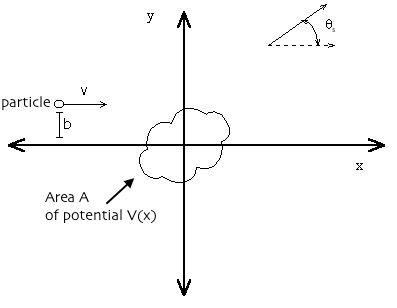
\includegraphics[width=0.5\linewidth]{SchemOfScattering}
		\caption
		[Schematic of Scattering Problem]
		{Schematic illustration of a scattering problem in two dimensions taken from \cite{chaoticIntro}.}
		\label{fig:SchemOfScattering}
	\end{center}
\end{figure}

This paper examines the scattering problem in two dimensions with four Gaussian potential hills instead of the one arbitrary potential bounded by a region. Additionally, the Gaussian potentials are that of gravity, hence the model simulates a particle rolling through a plane with four identical hills placed around one point. The model is discussed in further detail in Section~\ref{sec2:PhysicsModel}.




%----------------------------------------------------------------------------------------
%	Physics Model
%----------------------------------------------------------------------------------------



\section{Physics Model} \label{sec2:PhysicsModel}



\subsection{Description of the Model} % Sub-section


\begin{figure}[H]
	\begin{center}
		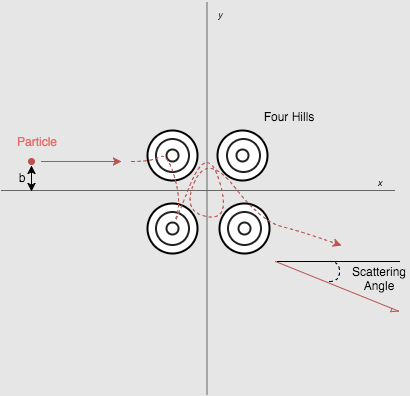
\includegraphics[width=0.5\linewidth]{scattering4HillSchem}
		\caption
		[Schematic of Scattering with Potential Hills]
		{Schematic illustration of the scattering problem with four potential hills in the particle's path. $b$ is the initial $y$ position of the particle, and is known as the impact parameter. The scattering angle is made by the particle's trajectory with the horizontal axis. The dashed line shows the trajectory of the particle.}
		\label{SchemOfScattering}
	\end{center}
\end{figure}


Section~\ref{Intro:SimpleExample} discussed a scattering model with one potential. Using that, consider a particle moving towards a potential $V(x,y)$ without friction. This region's potential is different from the one mentioned in the previous section, as it is comprises four hills that have peaks at $(x,y) = (\pm 1, \pm 1)$. This system is shown in Figure~\ref{SchemOfScattering}. 

 As seen in Figure~\ref{SchemOfScattering}, the particle initially starts at a fixed horizontal distance, sufficiently far from the potential, so that it is unaffected by the dynamics due to the potential. Its vertical distance from the $x$ axis is denoted as $b$, and is called the `impact parameter.' This impact parameter is what defines the point of entry of the particle into the region with the potential, known as the scattering region. \\
 
 
 After interacting with the scattering region, the particle exits the area, its trajectory forming an angle with the $x$ axis. This angle is known as the scattering angle, and is the same as the one mentioned in Section~\ref{Intro:SimpleExample}.\\

It is expected that if the energy $E$ of the particle is greater than the maximum potential energy at the hill peaks $E_m$, then the particle should be able to pass through the hilly region without much alteration in its trajectory, and the scattering is non-chaotic \cite{GRice}. While decreasing $E$ below the threshold energy $E_m$ and altering $b$ in small increments, we expect the scattering angle to vary unpredictably, demonstrating the chaotic nature of the system \cite{GRice}. The functional dependence of the scattering angle and the impact parameter is interesting because it is different for the regions where the scattering is chaotic and where the scattering is non chaotic. This is discussed further in Section ~\ref{Results:chaoticVsNon}.\\





\subsection{Physical Theory}


Here, we will discuss the physics behind the dynamics of the system. We start by studying the the equation for the potential mapped by our four hill system, 
\begin{equation} \label{potentialEq}
\vec{V}(x,y) = x^2 y^2 \ e^ {-x^2-y^2}.
\end{equation}
\noindent This potential, as seen in Figure~\ref{potHills}, is what causes the trajectory of our particle to deviate as it enters the scattering region. The reason the deviation actually occurs is because the potential imposes a force on the particle, which causes the particle to accelerate to the region where the potential is the lowest.   

%label a and b 
\begin{figure}[H]
	\begin{center}
		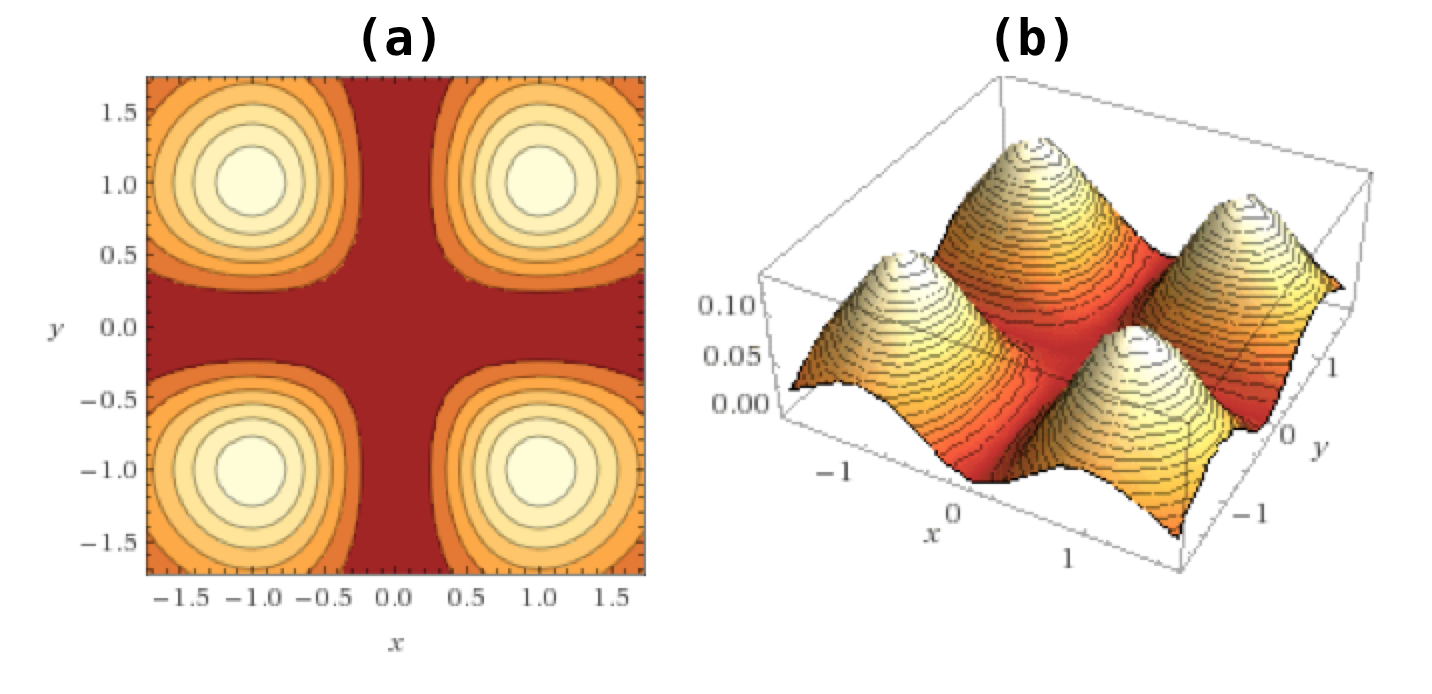
\includegraphics[width=0.7\linewidth]{potHillsWolfram}
		\caption
		[Plots of the Potential]
		{A contour plot (a), and a three-dimensional plot (b) created on Wolfram Alpha for the potential hills of equation~\ref{potentialEq}. 
			The potential has four maxima, at coordinates (1,1) , (-1,-1) , (-1,1) , (1,-1). At these maxima the potential energy has a value of $V(x,y) = 1/e^2 = E_{max}$.}\label{potHills}
	\end{center}
\end{figure}


We know from the laws of energy that a force is equal to the negative gradient of a potential, or $ \vec{F} = -\nabla \vec{V} (r) $ \cite{pang2006introduction}. Hence, we can calculate the force due to the potential given by equation~\ref{potentialEq} by finding its negative derivative :

\begin{equation} \label{ForceEq}
\begin{split}
\vec{F} &= -  \nabla \vec{V} (r)  \\
&= - \{2 e^{-x^2-y^2} x (-1+x^2) y^2,\ 2 e^{-x^2-y^2} x^2 y (-1+y^2)\}
\end{split}
\end{equation}

According to Newton's laws, we have $\vec{F} = m \vec{a}$, hence we can state that for a unit mass $m = 1 \ \text{unit}$, $\vec{F} = \vec{a}$ \cite{pang2006introduction}. In our system, we consider the particle as a unit mass, so the acceleration of the particle in the scattering region is 

\begin{equation} \label{ForceEq}
\begin{split}
\vec{a} = - \{2 e^{-x^2-y^2} x (-1+x^2) y^2,\ 2 e^{-x^2-y^2} x^2 y (-1+y^2)\}.
\end{split}
\end{equation}




With this formula, we can use different numerical integration techniques to calculate the evolution of the position of our particle over time as it traverses through the scattering region. Note that the idea of using a unit mass to make calculations simpler was taken from a program written to simulate two celestial bodies in \cite{pang2006introduction}. 



%----------------------------------------------------------------------------------------
%	Numerical Integration
%----------------------------------------------------------------------------------------




\section{Numerical Integration and Computation Accuracy }  \label{Sec3:NumericalInt}% Major section

\subsection{Integration in Simulations}

There are various ways to calculate the area underneath the curve of a function, and thereby estimate the value of a definite integral. One way is the by the `Midpoint Rule.'



Consider the following integral $\int_{a}^{b} f(x) dx$, where $[a,b]$ is the interval of integration, $f(x)$ is the function being integrated, and $dx$ is a small width that is the length of each subinterval. We calculate  midpoints between the points separated by the distance of $dx$, and then evaluate the value of $f(x)$ at these midpoints, as seen in Fig~\ref{fig:integral}. 

%label a and b 
\begin{figure}[H]
	\begin{center}
		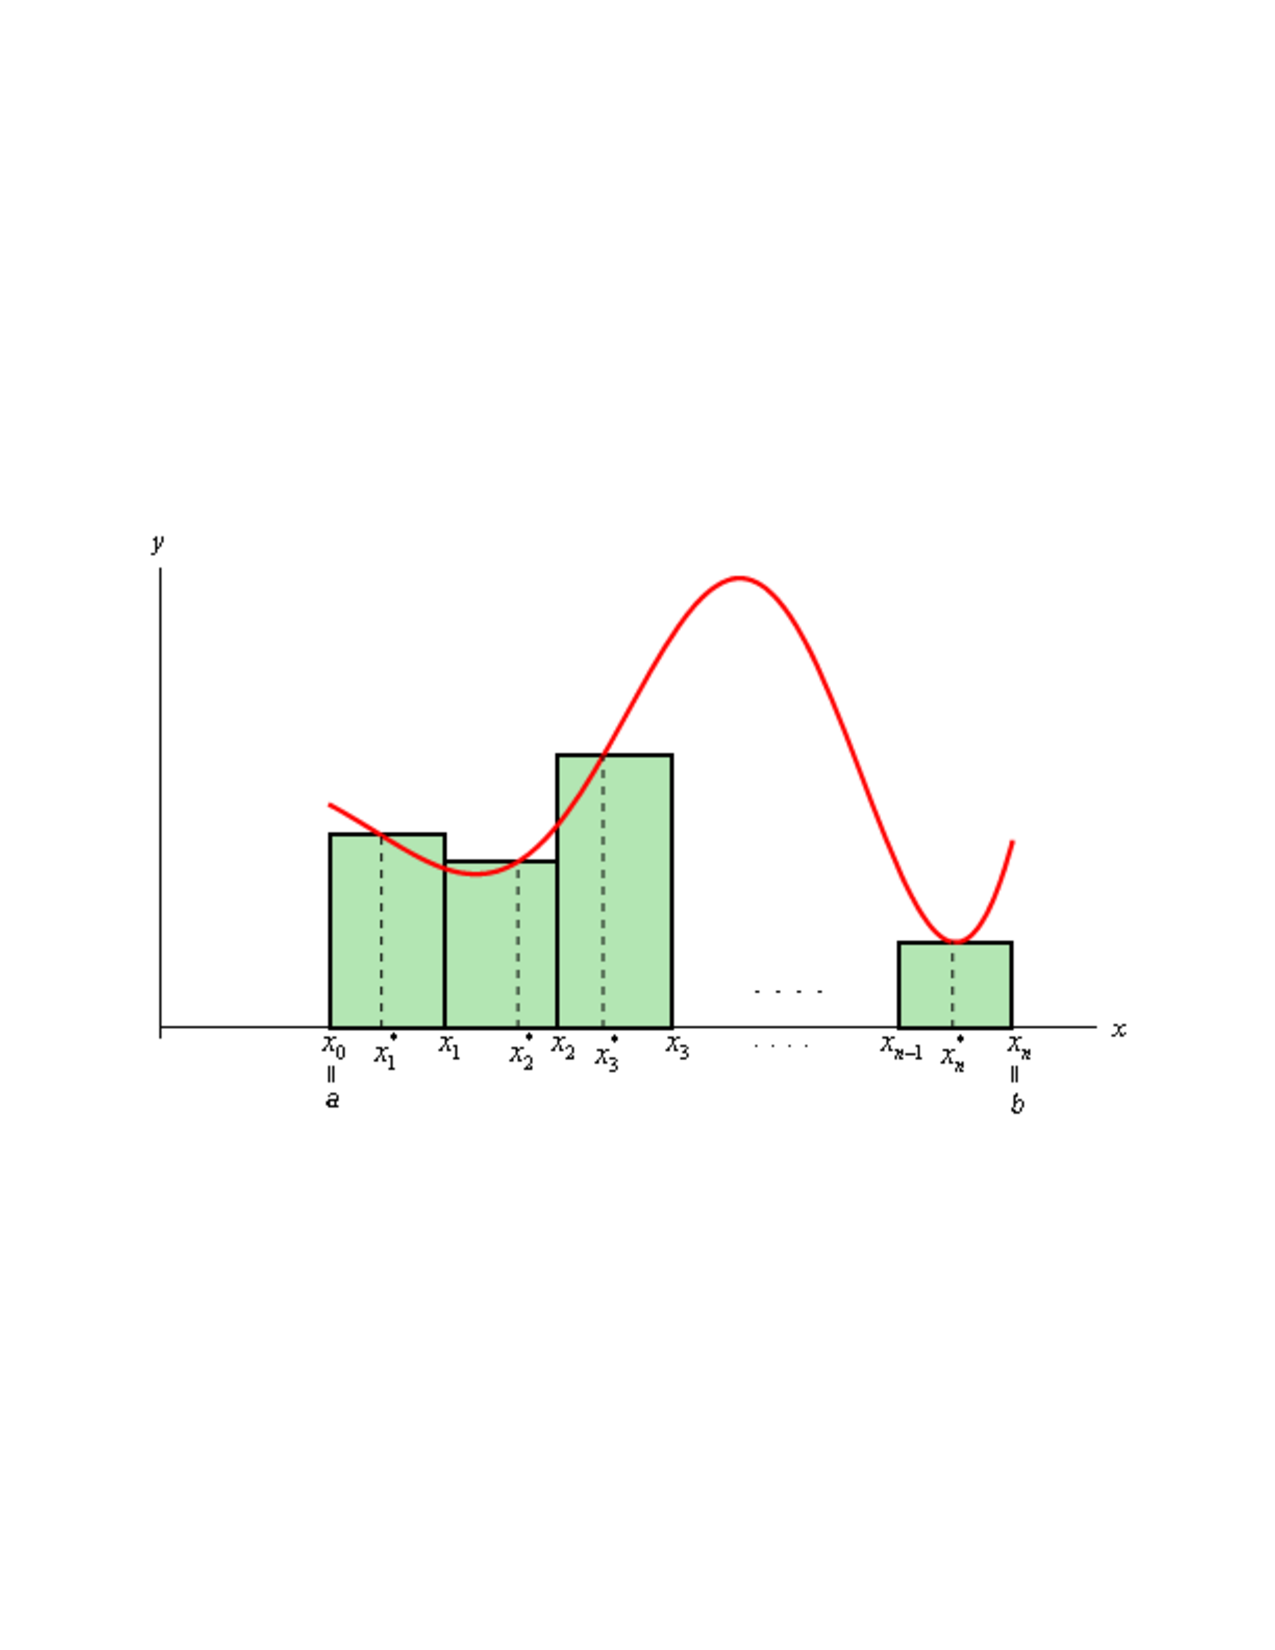
\includegraphics[width=0.7\linewidth]{integral}
		\caption
		[Midpoint Rule for Integration]
		{An integral being evaluated with the midpoint rule. The distance between intervals $[x_1, x_2], [x_2, x_3]...$ is $dx$, and the midpoints of these intervals are $x_1^*, x_2^*...$ These midpoints are where $f(x)$ is evaluated.}
		\label{fig:integral}
	\end{center}
\end{figure}

As seen in the graph, we can break the area underneath the curve of $f(x)$ into several rectangles.  Each rectangle has a width of $dx$, and a height equal to the value of the function, $f(x)$, evaluated at the midpoints of the rectangles. Summing the areas of each of these rectangles, we can estimate the value of the definite integral.\\

This process of integration is very similar to what is used in the simulation. However, instead of using the `Midpoint Rule,' the simulation uses the Euler-Cromer, and Runge-Kutta algorithms, which use different methods for obtaining the midpoint. \\

Additionally, the subintervals for integration in this simulation are $dt$, known as the time step. This is the size by which the time variable $t$ is increased before evaluating the value of the function at time $t$.


\subsection{Varying the Size of Time Steps}

 

A brute force method to increase the accuracy of computations in most physical experiments is simply to take data for a larger number of points. For computational experiments such as this one, the number of data points can be increased by decreasing the size of $dt$, the time step used for integration, while still integrating over the same period of time \cite{computationalText}. However, this technique makes computations much slower, because more calculations are required \cite{computationalText}. \\

Additionally, many computational physicists use variable time steps to increase integration accuracy and speed. In this simulation a variable time step is set up so that the time step becomes smaller as the speed of the particle increases. By doing this, the simulation maps the path of a particle to a more accurate degree as it travels at higher speeds. Speed increases are more likely to occur as the particle takes sharp turns. The variable time step also allows the computations to be fast, since in regions where the particle's speed is relatively constant, the time step becomes larger. This speeds up the computation while still accurately recording data for the position of the particle. \\

Another method to increase accuracy is finding and using better suited and more efficient algorithms for the computations. In the following section, we will discuss some numerical integration algorithms that we use for the chaotic scattering simulation. 


\subsection{Numerical Integration Techniques}


Here we discuss the various numerical integration techniques that we can use to calculate the evolution of the position of our particle with time as it traverses through the scattering region as discussed earlier. Before we begin talking about numerical integration techniques, we first provide a background on these techniques.

\subsubsection{What is Numerical Integration?}

 Newton and Libniz discovered calculus, and demonstrated to the world a vast new set of mathematical possibilities \cite{ODE}. However, mathematicians discovered some ordinary differential equations that could not be solved using techniques provided by Newton and Libniz. \\


 An ordinary differential equation (an ODE) is a function that expresses the rate of change of a function with respect to changing variables \cite{ODE}. For example, a common type of ODE that we encounter can be expressed as $f (x, y) = dx /dy$. To solve such differential equations, mathematicians try to obtain the original function, which creates a specific rate of change with certain initial values for the variables. \\

 Although representing ordinary differential equations in this manner makes solving them seem trivial, there are many ODEs that cannot be solved with algebra and integration. In order to solve these types of ODEs, mathematicians such as Euler, Runge and Kutta began looking at the use of small estimations to approximate the path that a function followed \cite{ODE}. Hence, these methods provide us with approximations for solutions of differential equations. This process, known as numerical integration, immediately proved to be a invaluable tool for mathematicians. With numerical integration, we can approximate many more ODEs and thereby have the ability to measure the rate of change of various functions, such as temperature changes, population growth, and even velocity \cite{ODE}. \\
 

 Because of the usefulness of numerical integration, many mathematicians have worked on forming different techniques for it. Additionally, since the behavior of each ODE varies,  different numerical integration methods are required to undertake different problems. This consequently gives rise to many mathematicians creating their own numerical integration techniques, each having their own costs and benefits \cite{ODE}. \\

We now discuss two popular numerical integration techniques used to calculate quantities such as the trajectories of astronomical bodies. These are the techniques that have been used in our simulation to calculate the trajectory of the particle.


%------------------------------------------------
\subsubsection{Euler-Cromer} \label{NumericalInt:EulerCromer}

%  http://supercomputingchallenge.org/07-08/finalreports/82.pdf


In the late 18th century, Leonhard Euler, the man who discovered the famous relation, $e^{ \i \pi} = -1$, was also one of the mathematicians of his time to recognize the beauty of numerical integration \cite{comparingODE}. With his studies, he produced a simple numerical integration technique. The numerical integration method works by first calculating the slope at a given point, and then recalculating it after stepping over a fixed interval \cite{ODE}. These can be easily calculated if an initial starting point is given. This process is then repeated at a new point. Plotting the slopes calculated at the different points helps us approximate the graph of the original function from which we obtained the ODE. \\

In the case of the chaotic scattering problem, we have a differential equation defining the acceleration of the particle as the second derivative of the position of the particle as seen below \cite{computationalText}. 
$$ a (t) = \frac{d^2}{dx^2} x(t)  $$

 This equation can be broken into two differential equations, relating position $x(t)$ to its derivative, velocity $v(t)$ and relating velocity to its derivative, acceleration $a(t)$:


$$ x_{n+1}(t) = x_{n}(t) + v_{n}(t) \triangle t$$
$$ v_{n+1}(t) = v_{n}(t) + a_{n}(t) \triangle t$$


These coupled differential equations can then be solved simultaneously using Euler's Method \cite{computationalText}. This process of calculating the position of a moving particle is very similar to how astrophysicists plot the trajectories of planets, and is what inspired this work \cite{computationalText}.\\

Cromer, a mathematician who was implementing this method, altered the process by first updating the velocity, and then the position (using the newly calculated velocity) \cite{comparingODE}. This means that the position is determined based on a later velocity, and hence is more accurate than the method Euler created. This modified method is known as the Euler-Cromer method. \\


Fig~\ref{fig:eulerCromer} contains the code for the implementation of the Euler-Cromer algorithm. 


\begin{figure}[H]
	\begin{center}
		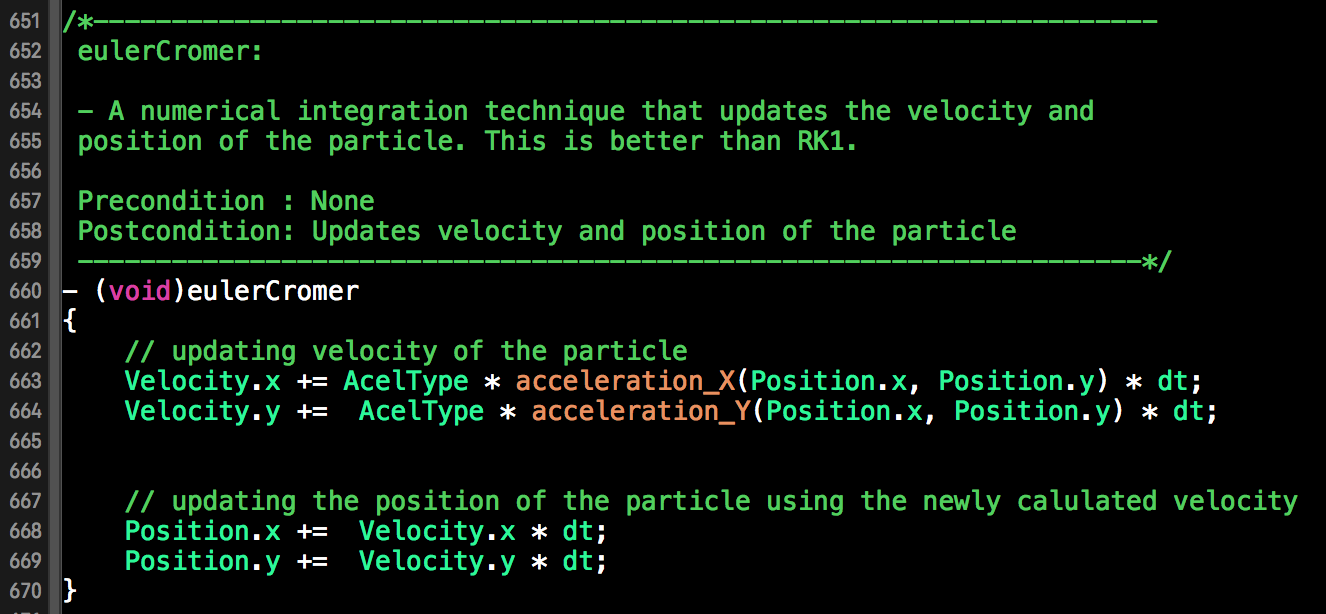
\includegraphics[width=0.7\linewidth]{eulerCromer}
		\caption
		[Code for Euler-Cromer Integration]
		{Implementation of the Euler-Cromer algorithm in the simulation. As seen, we are updating the velocity, position and then the time.}
		\label{fig:eulerCromer}
	\end{center}
\end{figure}







%------------------------------------------------
\subsection{Four Stage Runge-Kutta} \label{NumericalInt:RK4}



 A century after Euler created his numerical integration algorithm, Carl David Tolmé Runge and Martin Wilhelm Kutta created a new set of numerical integration schemes known as the Runge-Kutta methods \cite{comparingODE}. Like the Euler-Cromer algorithm, sets of numerical integration techniques can be applied to a large set of problems. These methods calculate each point by first calculating trial steps at the mid point of the time step \cite{OldRunge}. These midpoints help remove lower-order error terms, and make the calculation of each point more accurate, as the point is calculated by taking the average of several midpoints, each with different weights \cite{OldRunge}.\\
 
 As you increase the order of the Runge-Kutta method, you get more mid points. Hence the higher the order of the Runge-Kutta method, the more the number of mid points that we use to calculate the value of one data point \cite{OldRunge}. This makes the approximation more accurate; however, it also makes the time taken for the approximation longer. Additionally, since the number of mid points that are present between a time step increases as we increase the order of the Runge-Kutta method, the higher order algorithms can be accurate even with a large time step \cite{OldRunge}. \\
 
 The most popular Runge-Kutta method is the forth order method, known RK4. The RK4 method is preferred since it has a higher degree of accuracy than the lower order algorithms, but at the same time does not take as long as other higher order algorithms \cite{OldRunge}. The step code for the Runge-Kutta 4 algorithm, along with the implementation of the code for this algorithm can be found in Appendix~\ref{RK4}.\\
 
 
 
%------------------------------------------------


%--------------------------------------------------

\subsection{Integration Accuracy Checks}
\label{Section:IntegrationAccuracyCheck}

As this is a system in which there are no external forces, energy is contained in the system. Hence, this provides us with a convenient tool to study the accuracy of integration: the energy of the particle. If the energy of the particle is constant, then we know that the integration is accurate. We calculate this energy by summing the potential energy and the kinetic energy of the particle at a given point. The total energy is given by 

$$ Energy = \frac{1}{2} \ mass \cdot velocity^2(x,y) + potential(x,y),$$

\noindent where $potential(x,y)$ is the potential energy of the particle, as described in equation \ref{potentialEq}.


%----------------------------------------------------------------------------------------
%	Software
%----------------------------------------------------------------------------------------

\section{Software} \label{Sec4:Software}% Major section
Here, we discuss the software used to implement the model of the simulation. \\



%------------------------------------------------
\subsection{Programming Language and APIs} \label{Prog Lang and APIs}


We implement the model discussed in section \ref{sec2:PhysicsModel} in a Coca application for OS X. The program is in Objective C, and we rely on the various tools available via the Coca API to run it. Xcode is the IDE we use to construct the simulation, as it provides a straightforward interface builder, which permits users to easily connect buttons, text fields, and other items in the interface to back-end functions that make them work. 


%------------------------------------------------
\subsection{Interface Design and Interacting with the Program} \label{Intf Design+Interacting w program}

The application consists of a window with a view of a two-dimensional plane, displaying the four hills, and the particle at a distance from the hills, as seen in Figure~\ref{fig:choas}. The trajectory of the particle can be adjusted by clicking on the view, and dragging the initial path of the particle along the $y$ axis. Alternately, the starting position of the particle can be set within the `Initial Y (b)' text field. The `b' is the symbol for the impact parameter used in comparable simulations for chaotic scattering. As discussed earlier, it is this variable that causes chaotic scattering at certain values.  \\


\begin{figure}[h]
	\centering
	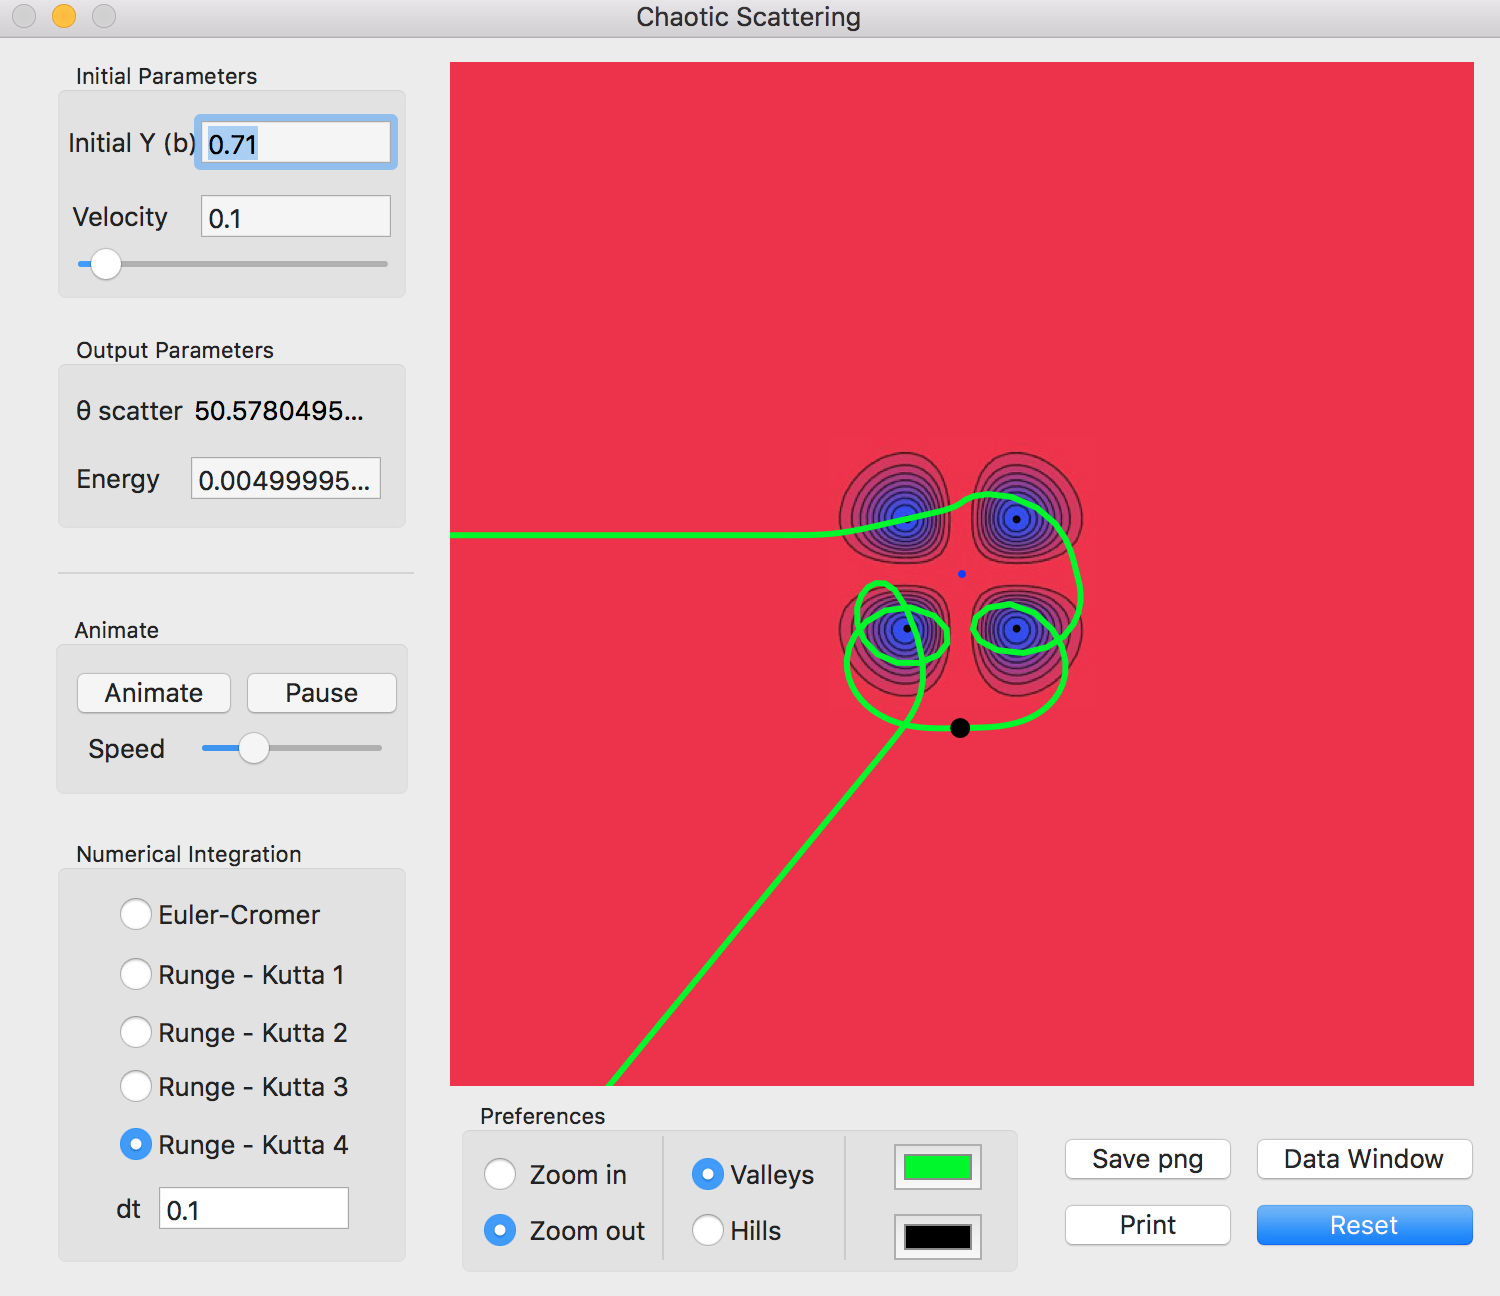
\includegraphics[width=0.8\textwidth]{image1.png}
	\caption
	[Screen Shot of Application 1]
	{A screen shot of the application. The blue lines represent the potentials of the system while the green line traces the path of the particle. }
	\label{fig:choas}
\end{figure}


The particle's velocity, another input parameter, can be changed within the text field marked `Velocity,' or with the horizontal slider underneath it. Changing this will in turn change the energy of the particle. Increasing the energy, or the initial velocity of the particle while keeping the `b' constant, can demonstrate how having a different velocity can cause different trajectories to emerge. This is discussed in Section \ref{CompVeltoAngle}.\\ 

The user may also change the numerical integration technique used to calculate the path of the particle by choosing between the radio buttons for the Euler-Cromer algorithm, and various Runge-Kutta algorithms. With this option, users can observe how numerical integration techniques alter the path of the particle.\\
 
Once the integration algorithm and input values are chosen, the simulation generates a path as shown in Figure~\ref{fig:choas} and \ref{fig:chaos2}. On clicking the `Animate' button, an animation of the particle traversing the potentials can be seen. \\

\begin{figure}[h]
	\centering
	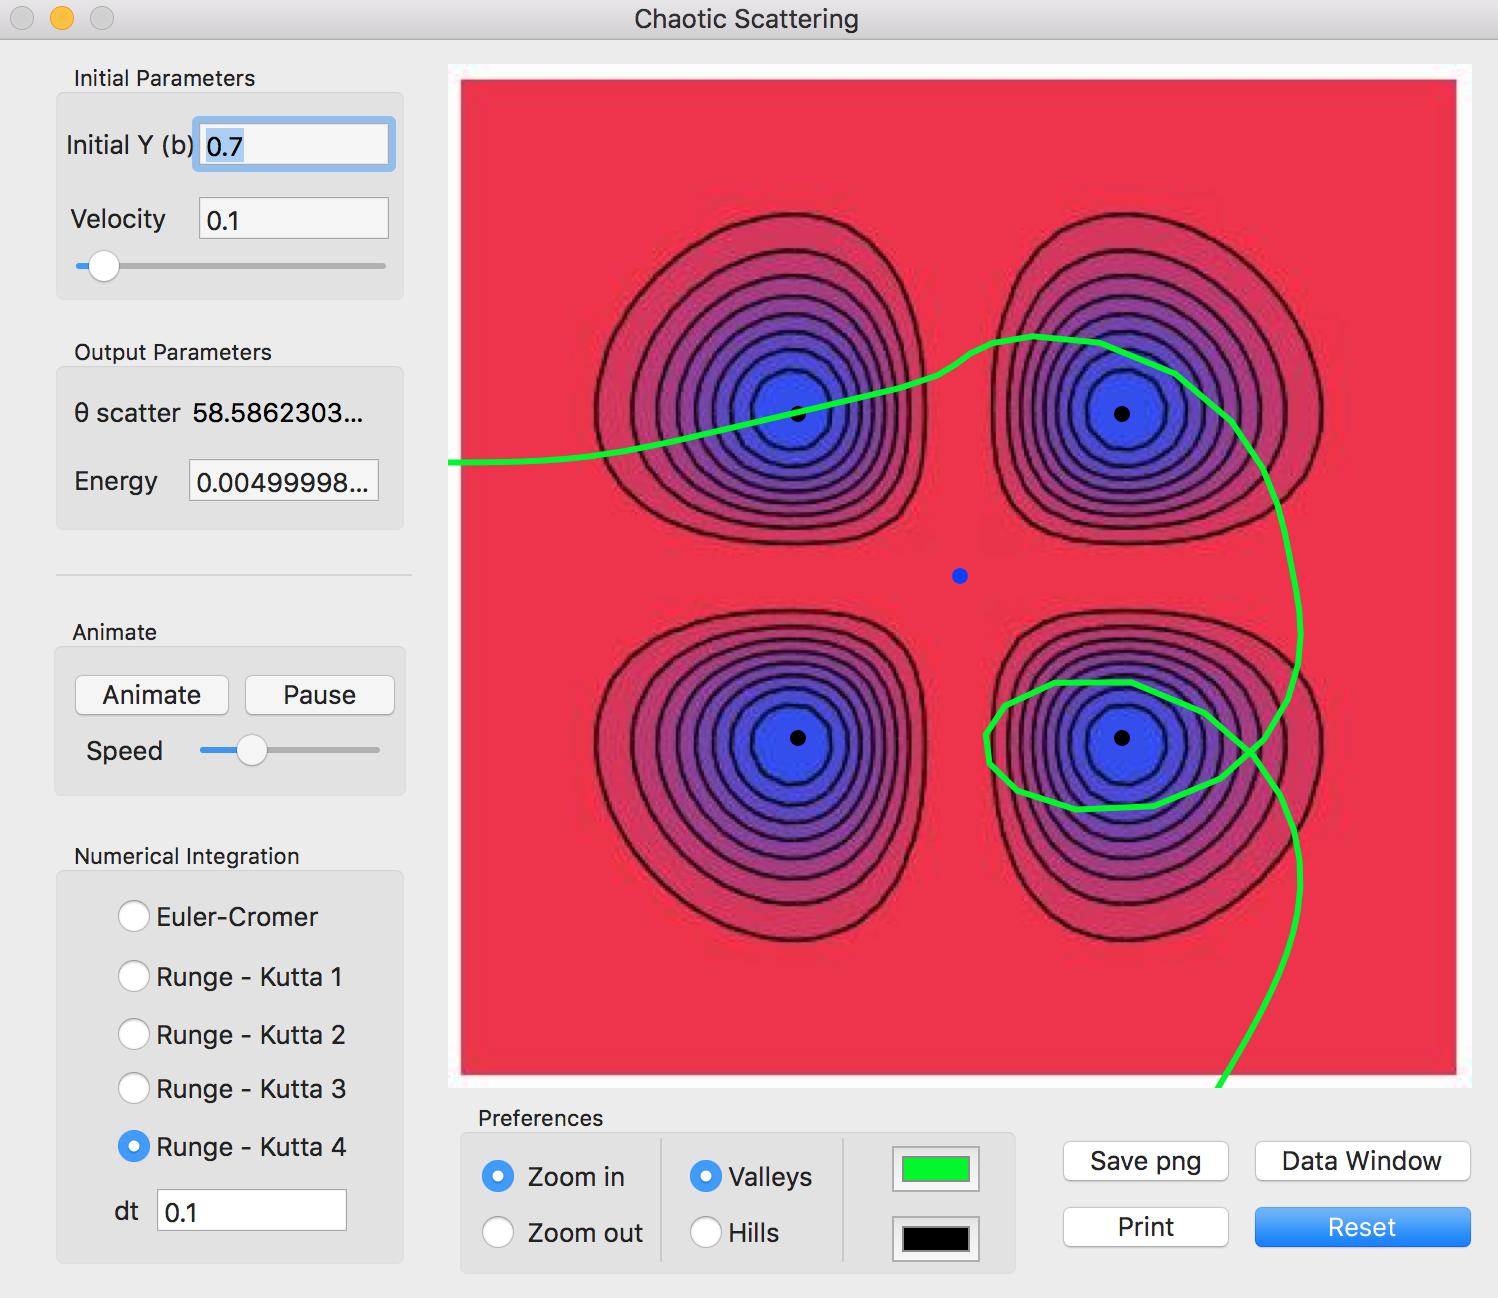
\includegraphics[width=0.7\textwidth]{image2.png}
	\caption
	[Screen Shot of Application 2]
	{A similar screen as in Fig~ \ref{fig:choas}, however with its initial $y$ position altered by a factor of 0.01. Additionally, this is a zoomed in version. This trajectory clearly differs by a great amount from the first one, displaying the chaotic nature of the system. }
	\label{fig:chaos2}
\end{figure}



After the particle finishes its transit through the hilly region, it exits the system at an angle from the $x$ axis. This angle is the scattering angle and is displayed in the the `$\theta$ scatter' text field. Below that text field, the energy of the particle as it exits the system is displayed. \\


The `Data Window' button opens a new window as seen in Figure~\ref{fig:DataArchivingWindow} with options for archiving data in text files. The `Archive Data for b' option runs the simulation for a set of initial $y$ positions and records the various scattering angles of the particle from the system. This data when plotted displays interesting fractal patterns. The `Archive Data for Velocities' runs the simulation for different initial velocities at the same $y$ position. Like the previous data run, this also records the scattering angle. The `Energy Data' button allows the user to save the value of the energy of the particle at each point in its path. This is useful to tell us if the integration is accurate or not.\\


\begin{figure}[h]
	\centering
	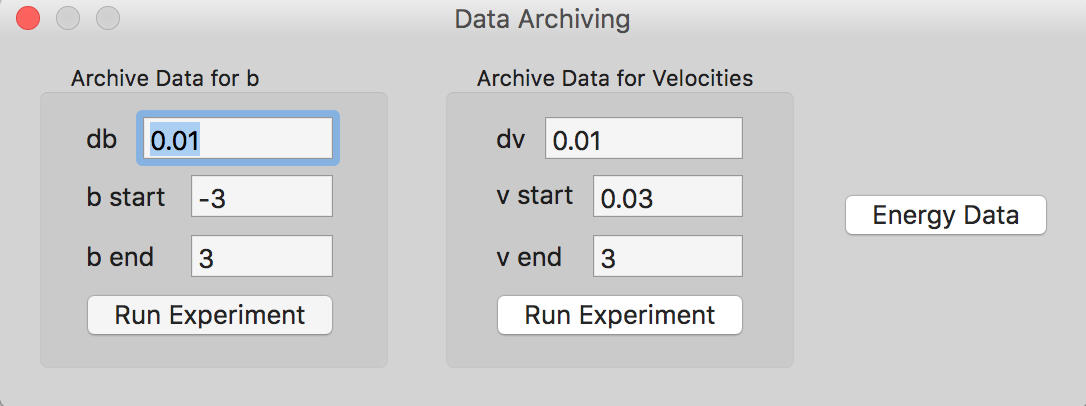
\includegraphics[width=0.6\textwidth]{dataWindow}
	\caption
	[Screen Shot of the Application's Data Archive Window]
	{The window for data archiving.}
	\label{fig:DataArchivingWindow}
\end{figure}


The most challenging portion of creating this program is determining the potentials of the four hills, and making the particle follow the potentials near the hills. Additionally, making the animation push a particle forward through the path was an intricate problem. However, the fact that this simulation provides new insights to the chaotic scattering problem makes the investigation worthwhile. Calculating the scattering angle was also confusing at first. The following section describes the process by which the program calculates the scattering angle. \\




\subsection{How the Scattering Angle is Calculated}

The program has a loop that starts the particle at an initial position off the screen. The distance between the position where the particle starts, and the center of the region with the hills, is used as the radius of a circle. In the program, the area enclosed by this circle is considered to be the entire universe where the particle can exist. After the particle leaves its initial point, interacts with the scattering region and exits the screen, it eventually reaches the boundary of its circular universe, which is present off the screen. The coordinates of where the particle touches the circle $(x,y)$ and the point right before it touches the circle $(p,q)$ are recorded and can be see in Figure~\ref{fig:scatteringAngleCalculation}. \\ 


\begin{figure}[h]
	\centering
	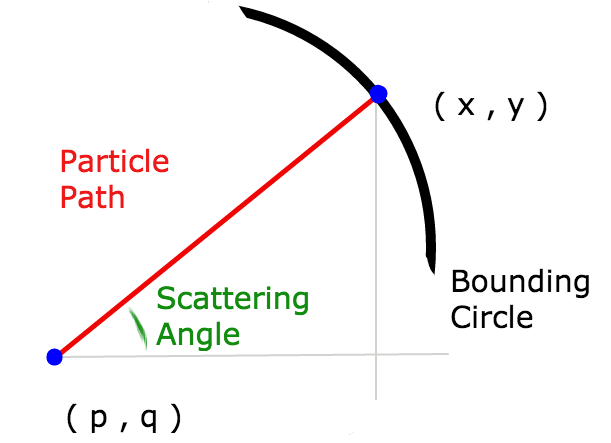
\includegraphics[width=0.5\textwidth]{Diagram.png}
	\caption
	[Diagram for the Scattering Angle]
	{The points (x,y) and (p,q) are the last two points of the particle's trajectory that are calculated. The bounding circle is the boundary of the simulation's universe. Using these two points, we can calculate the scattering angle.}
	\label{fig:scatteringAngleCalculation}
\end{figure}

With these values, we can calculate the scattering angle with the formula: 
$$ \theta_s = \tan ^{-1} \bigg(\frac{y - q}{x - p} \bigg) \ . $$



%----------------------------------------------------------------------------------------
%	Results and analysis
%----------------------------------------------------------------------------------------

\section{Results and Analysis}  \label{Sec5:ResultsAndAnalysis}% Major section



%------------------------------------------------

\subsection{Integration Accuracy Results}
As discussed in Section~\ref{Section:IntegrationAccuracyCheck}, by the law of energy conservation, the energy of the particle in the system  must remain constant at all times. Hence, we can consider only those trajectories where the particle has constant energy as physically realistic. On running the program at an initial $y$ position of $0.71$, and velocity of $0.1$, we discovered that the particle's energy remained constant with calculations made with the Runge-Kutta 4 algorithm. Hence, we concluded that this algorithm's calculations were the most accurate. We can see the plot of the energy in Figure~\ref{fig:EnergyZoom}.

\begin{figure}[h]
	\centering
	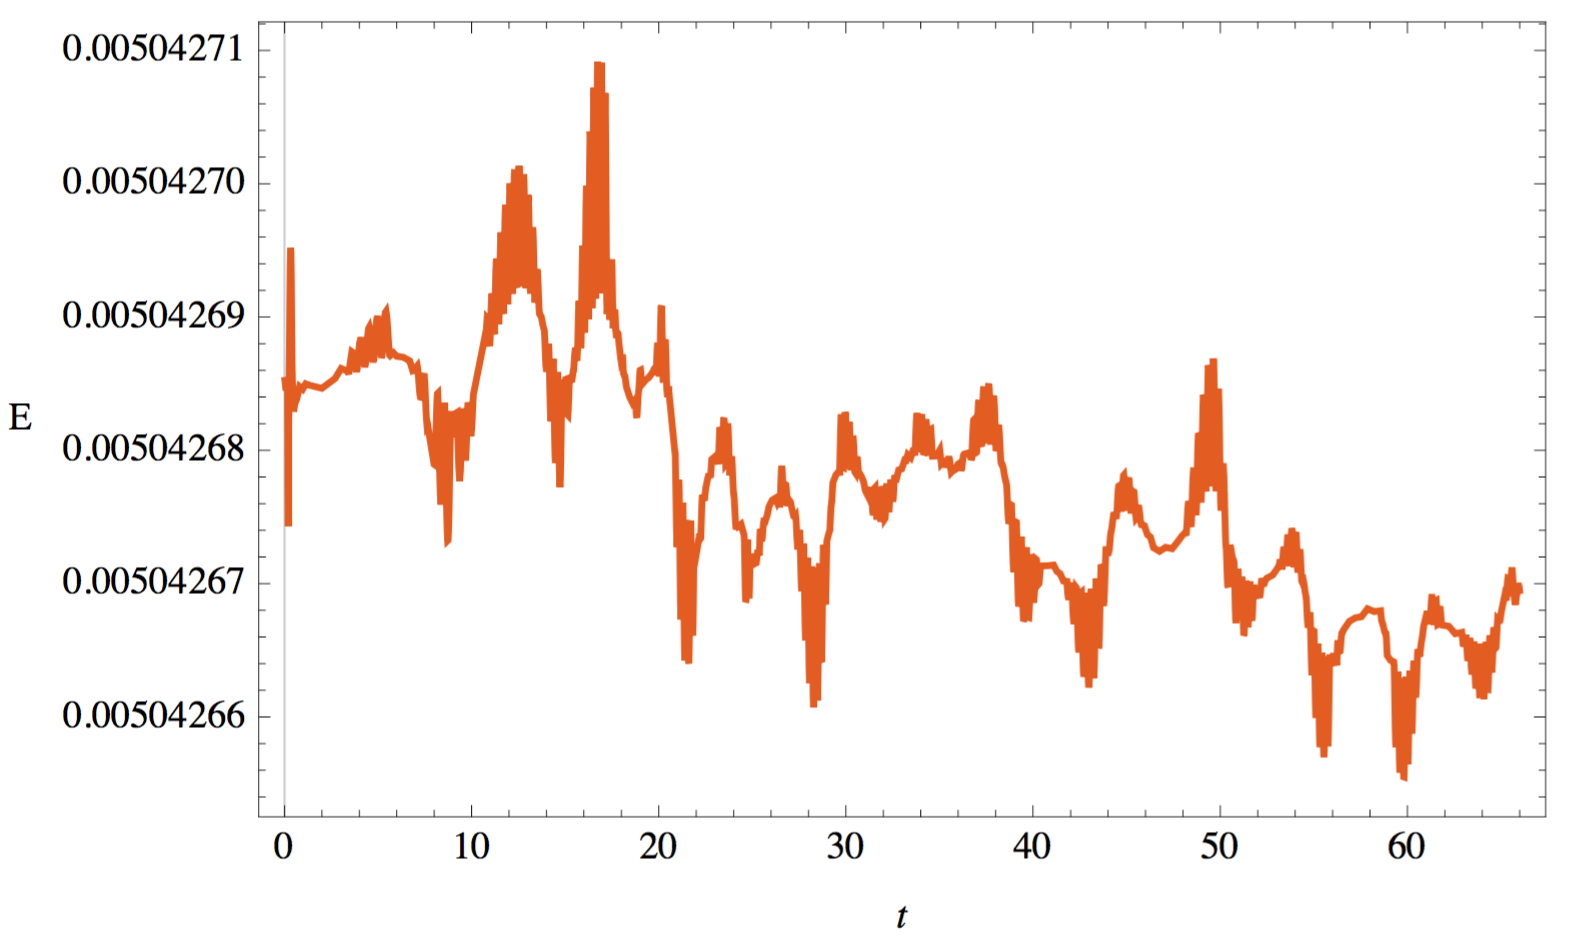
\includegraphics[width=0.6\textwidth]{Ezoom}
	\caption
	[Zoom in of an Energy Plot for the Particle]
	{A zoom in of the energy of the particle as it traverses through the scattering region. Although the energy appears to be fluctuating, it is not changing by a large enough amount to affect the trajectory of the mass. The path of the particle is calculated with Runge-Kutta 4.}
	\label{fig:EnergyZoom}
\end{figure}

Although this looks like the energy is fluctuating by large amounts, this is only because the graph's vertical scale is very small. If we increase the size of the vertical scale, we see that the energy remains constant, as seen in Figure~\ref{fig:Energy}.

\begin{figure}[h]
	\centering
	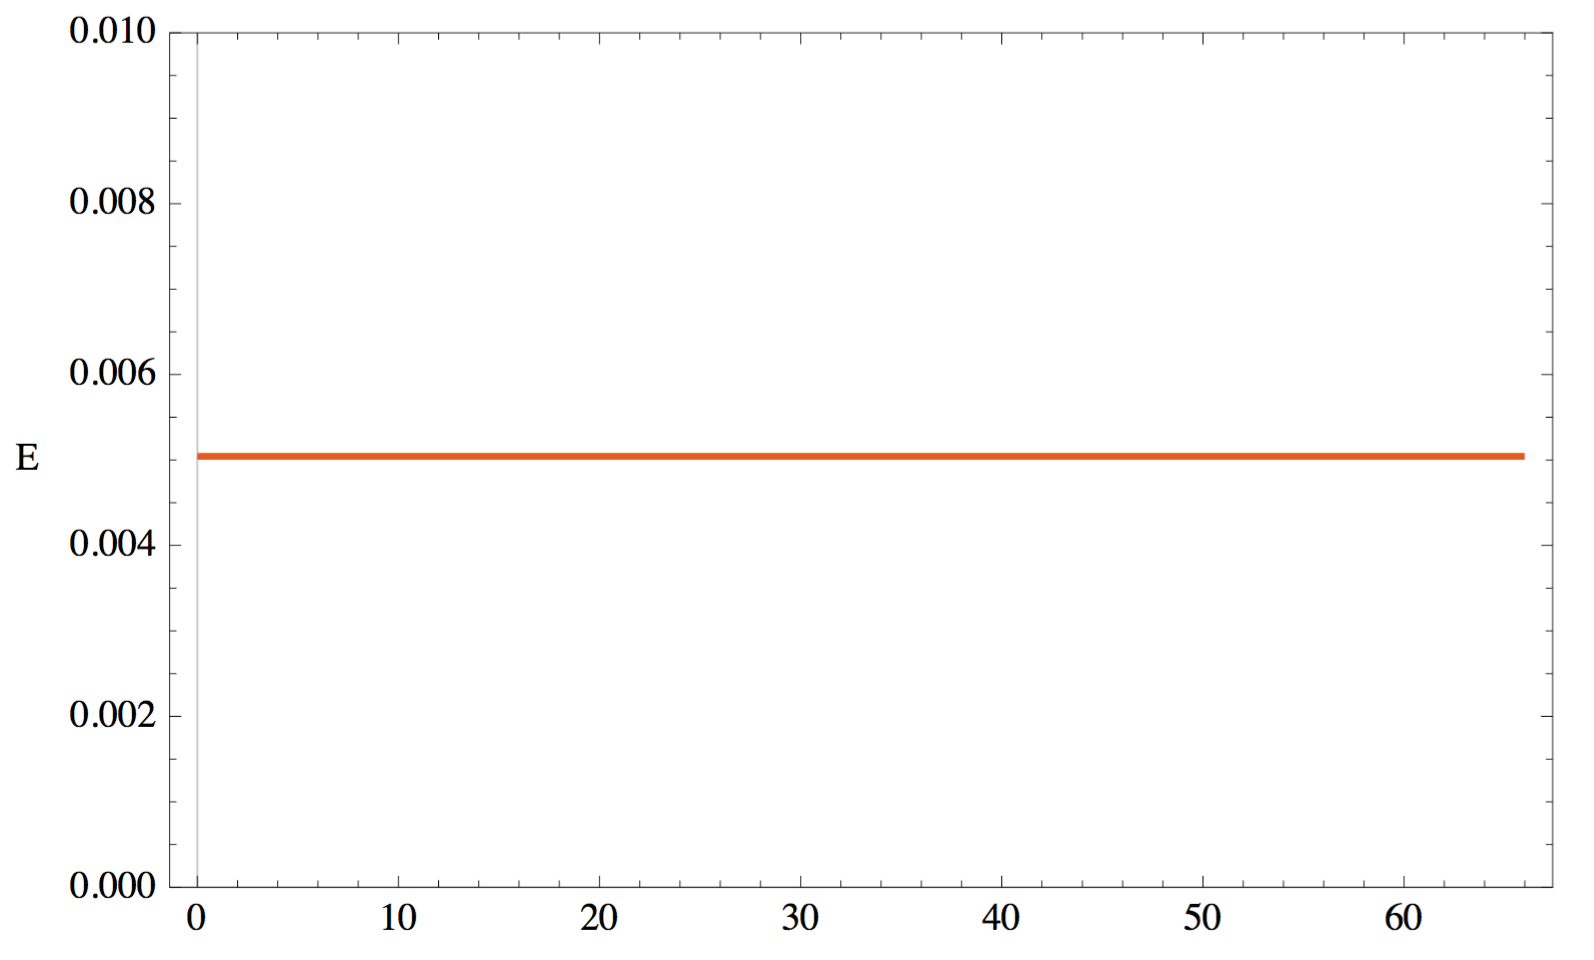
\includegraphics[width=0.6\textwidth]{E}
	\caption
	[An Energy Plot for the Particle]
	{The energy of the particle as it traverses through the scattering region. The path of the particle is calculated with Runge-Kutta 4.}
	\label{fig:Energy}
\end{figure}




Hence, as we were able to observe that the energy of the particle fluctuated by very small amounts with the Runge-Kutta 4 algorithm, these fluctuations would not affect the calculations on a relevant scale. Thus, we decided to take all of our data  using this algorithm.

\subsection{Chaotic, Non Chaotic and Fractal Regions in Plots} \label{Results:chaoticVsNon}




We ran the simulation and recorded the values of the scattering angle for impact parameters in the range $b=-5$ to $b=5$, with intervals of $b = 0.001$ and plotted the data in Figure~\ref{fig:thetaVSb}(a). From this plot, it is easy to distinguish between the nonchaotic regions--regions where the graph appears smooth (for example, between the range $b = -5 \text{ to } b = -3$)-- and the chaotic regions, the regions on the graph where there are great variations in small time steps. Looking at the nonchaotic region, we can see that increasing the impact parameter in this region does not alter the scattering angle by much. This is most likely because the path is not altered. On the other hand, looking at the chaotic regions, we can see that the scattering angle changes drastically with the impact parameter, and the graph appears to be fluctuating rapidly. \\ 



\begin{figure}[H]
	\begin{center}
		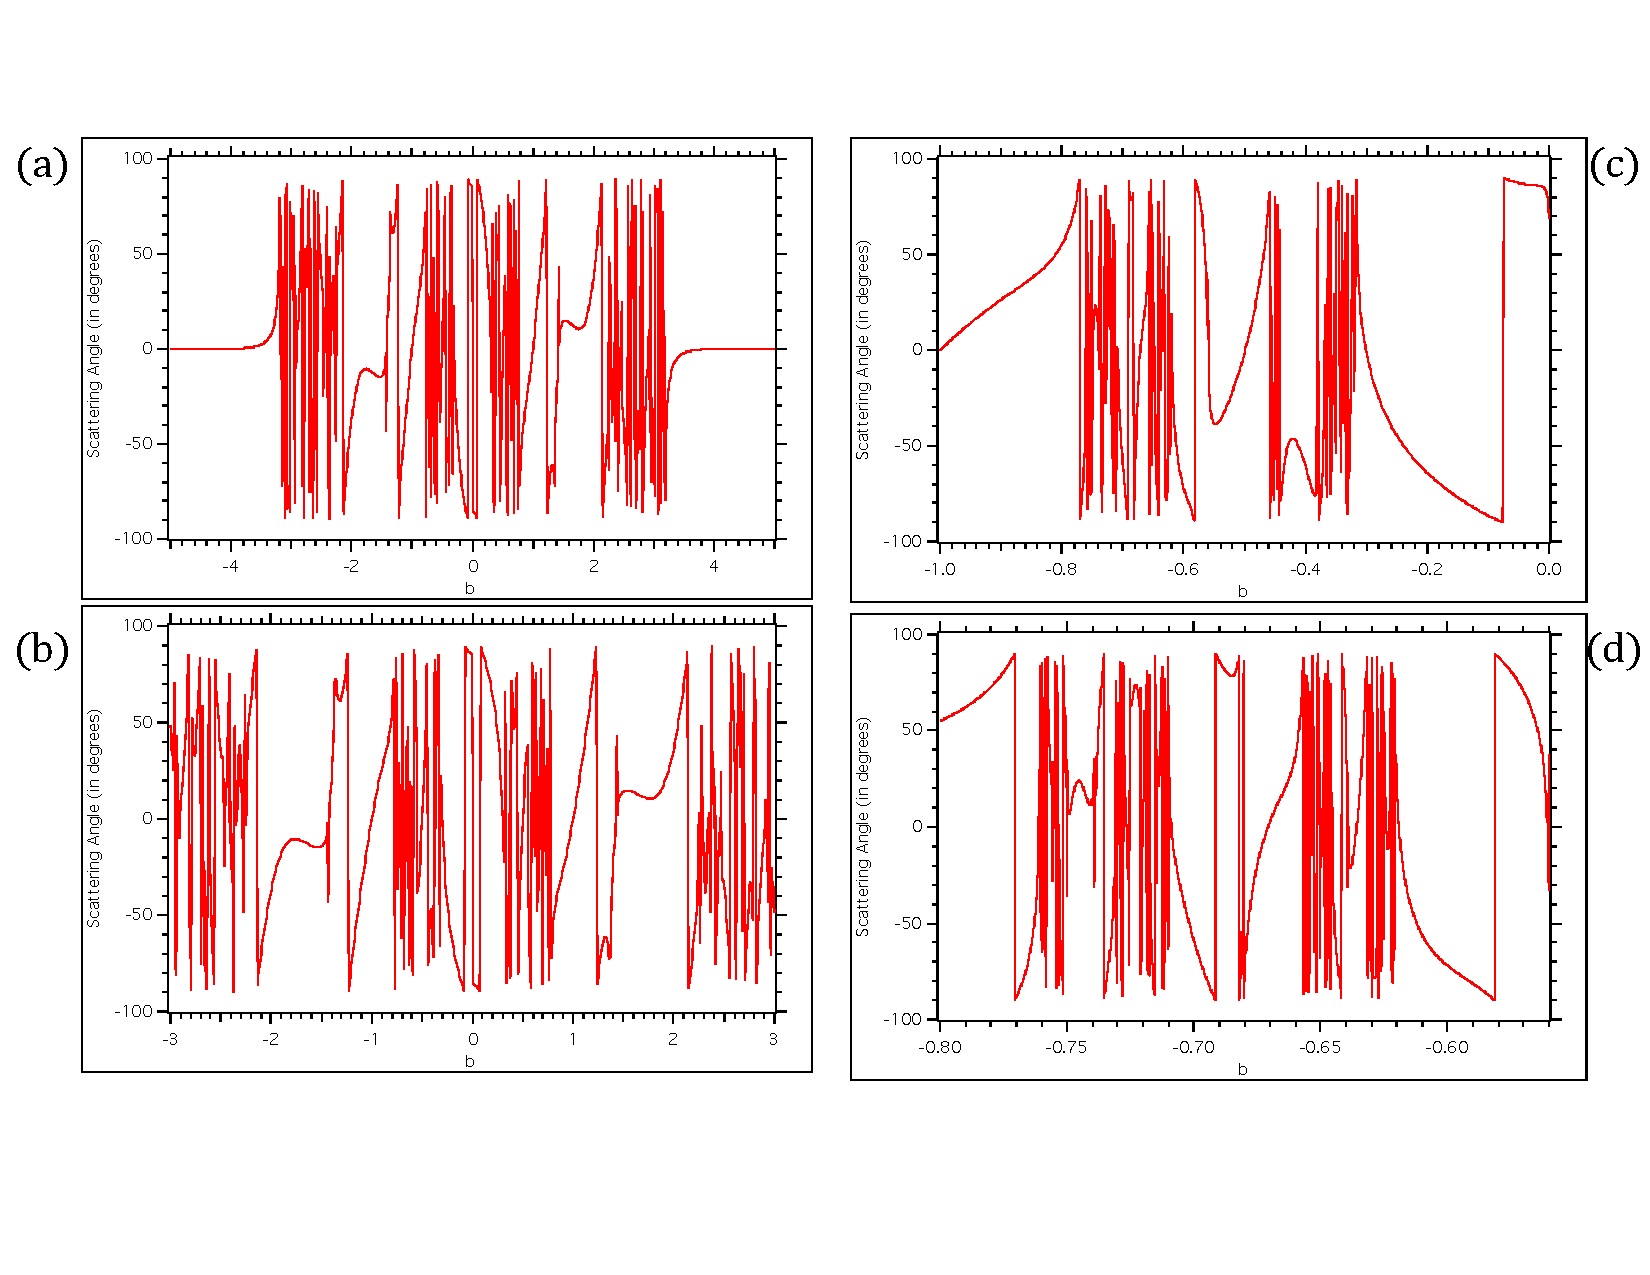
\includegraphics[width=1.1\linewidth]{AllGraphsTogether}
		\caption
		[Plots of the Scattering Angle VS Impact Parameter]
		{Plot (a) is of the scattering angle versus the impact parameter for a velocity of 0.10 . Plots (b), (c), and (d) show successive expansions of a small region in (a).}
		\label{fig:thetaVSb}
	\end{center}
\end{figure}


As it is difficult to clearly distinguish the pattern of this chaotic trend, we pick such a region and expand the graph along the horizontal axis as seen in Figure~\ref{fig:thetaVSb}(b), which shows the region between $b=-3\text{ to } b=3$. Clearly, the regions with rapid fluctuation still remain. Figures \ref{fig:thetaVSb}(c) and \ref{fig:thetaVSb}(d) show further expansions along the $x$ axis; however, even these still display fluctuating regions. \\ 

This suggests that there are ranges for the impact parameter for which the variations in the plots show a fractal nature. Quantitatively, what may be happening is that right before a region where the graph shows chaotic nature, the particle might have been interacting with two hills, and may have been looping around some of them, as seen in Figure~\ref{fig:choas}. A very small change in the impact parameter may have caused the particle to change the number of loops around the hills. This would be more than enough to drastically change the output parameter, which in this case is the scattering angle.\\




\subsection{Changing Initial Velocity for a Fixed Impact Parameter} \label{CompVeltoAngle}

\begin{figure}[H]
	\begin{center}
		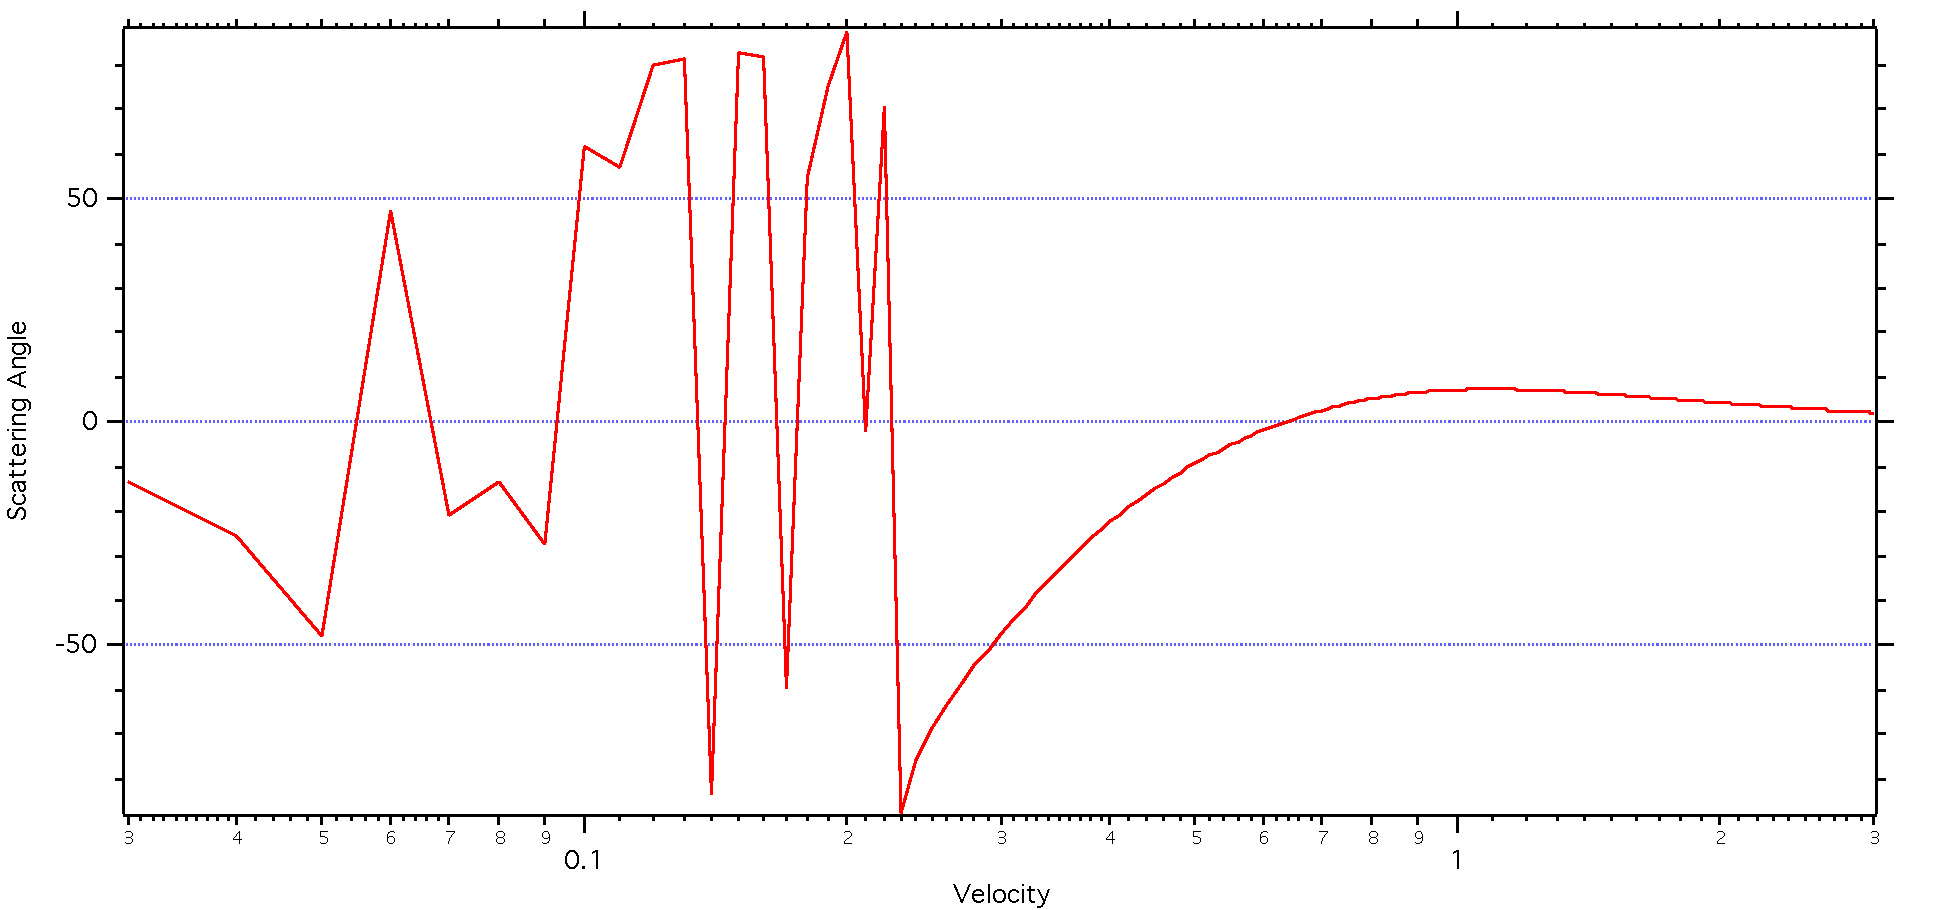
\includegraphics[width=1.1\linewidth]{ScatVSvel}
		\caption
		[Plots of the Scattering Angle VS Velocity]
		{Plot of the scattering angle versus velocity, for an impact parameter of $b=0.71$.}
		\label{fig:ScatVSvel}
	\end{center}
\end{figure}

We noted earlier that changing the velocity while keeping the impact parameter fixed changes the trajectory of the particle. To gain a better understanding of this phenomenon, we plotted the scattering angle against the velocity of the particle as seen in Figure~\ref{fig:ScatVSvel}. Studying the graph, we can see that at smaller velocities, the scattering angle changes rapidly. After a velocity of $0.23$, the scattering angle appears to increase gradually, and then as the velocity increases even further, the angle appears to gradually approach zero. This makes sense, as at higher velocities, the energy of the particle increases, and hence, it is less affected by the hills.




\subsection{Effect of Initial Velocity on the Scattering Angle}

\begin{figure}[H]
	\begin{center}
		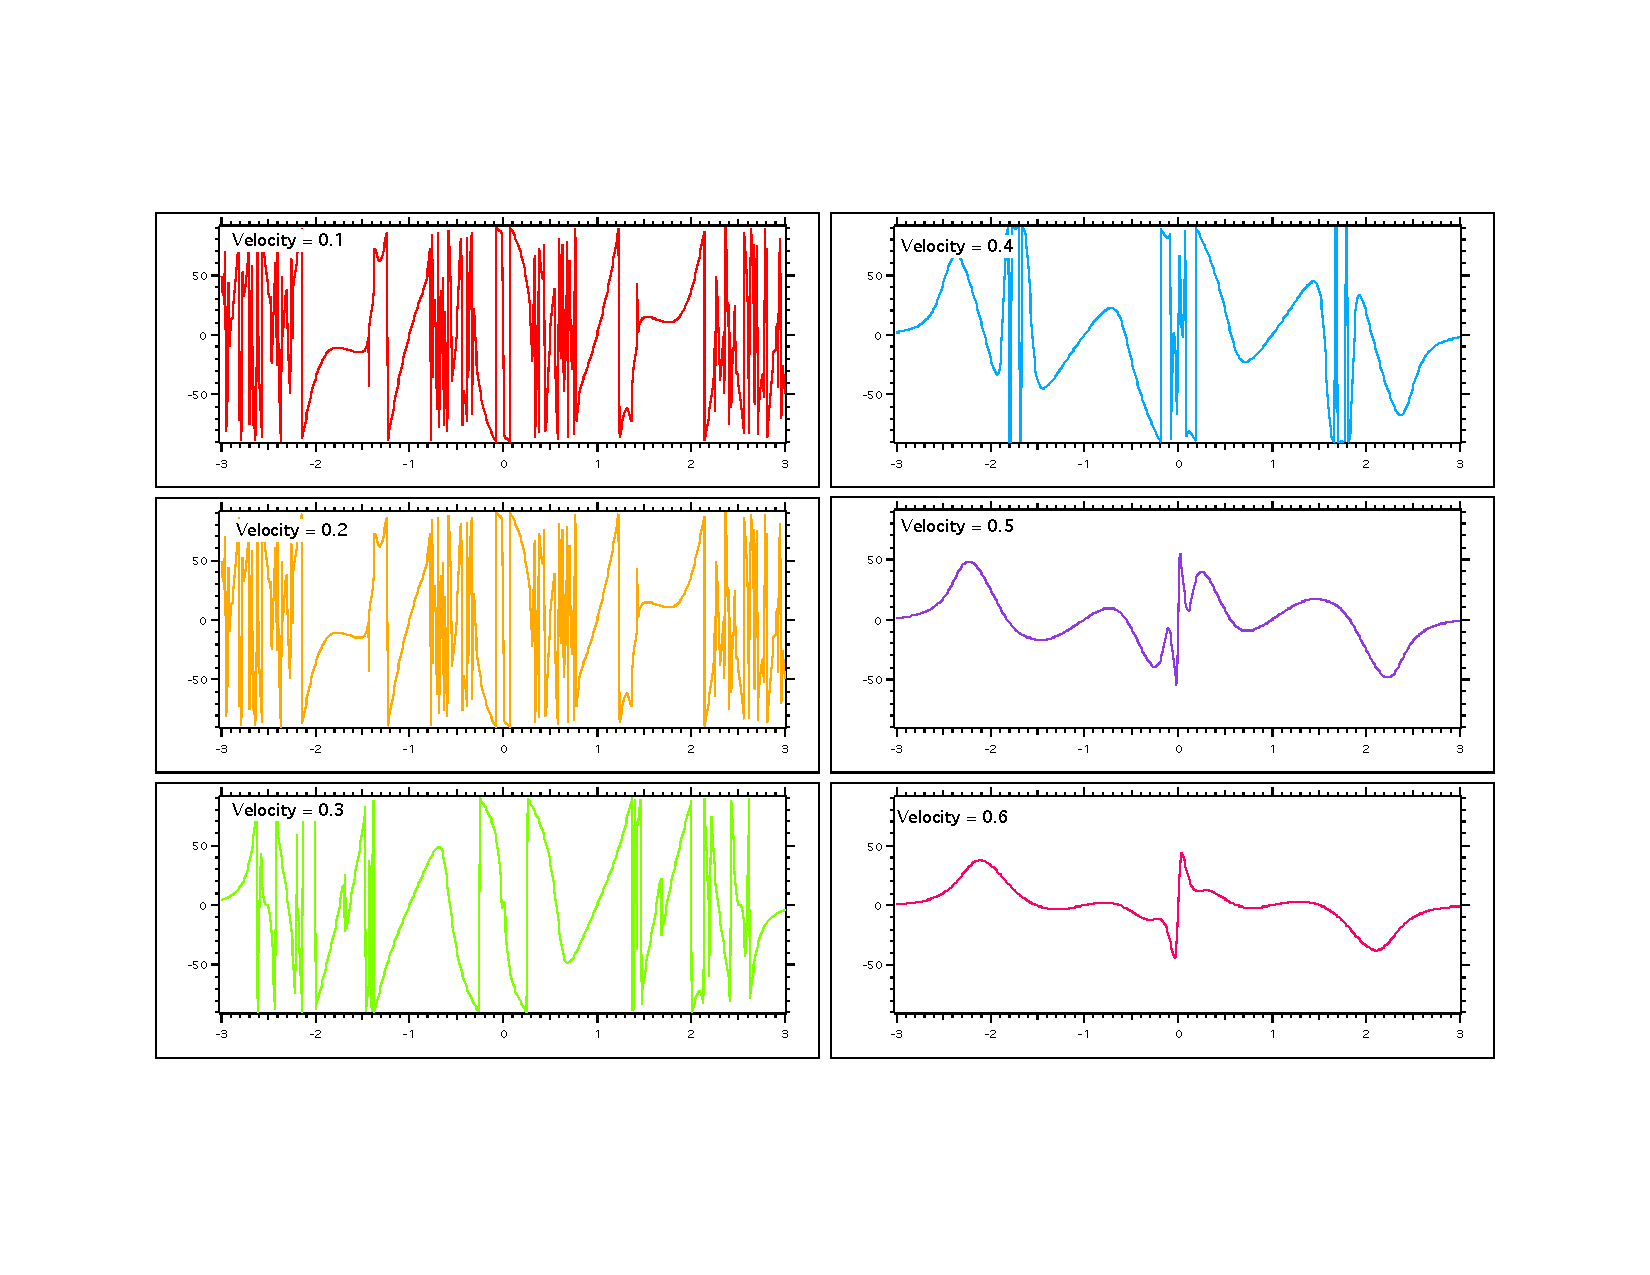
\includegraphics[width=1.1\linewidth]{bAtDifV}
		\caption
		[Plots of the Scattering Angle VS Impact Parameter for Different Velocities]
		{Plots of the scattering angle versus the impact parameter for velocities of $0.10$ to $0.60$.}
		\label{fig:bAtDifV}
	\end{center}
\end{figure}

We decided to study how changing the velocity affects the relationship between the scattering angle and the impact parameter. We plotted the data for velocities of $0.1$ to $0.6$, as seen in Figure~\ref{fig:bAtDifV}. These graphs are very interesting, as we can see that at certain velocities, there seems to be less chaotic nature. This makes sense as we know that at higher velocities, the energy of the particle is higher, and hence the particle is not affected by the scattering region at these velocities.




%----------------------------------------------------------------------------------------
%	CONCLUSION
%----------------------------------------------------------------------------------------

\section{Conclusions and Future Work} % Major section
Many new advances in the study of chaotic scattering have been made in the past decade. However, there is still much left to be understood from chaotic systems. Although we now have much more data than in the past, we still do not understand certain aspects of the dynamics in chaotic scattering regimes. There is still much work left to be done with this simulation as well. The next task a researcher could investigate is duration a particle spends within the scattering region. This is also supposed to have fractal properties in its data. After collecting data for both the time and the scattering angle, the researcher could possibly try to determine what is known as the `fractal dimension' of the system. With this, one can create an equation which helps describe fractal systems for chaotic scattering regimes. This could help further the studies of chaotic scattering and thereby help our understanding of various systems in nature. Recognizing the chaotic, fractal nature of our world can give us new insight, power, and wisdom. 
\newpage



%----------------------------------------------------------------------------------------
%  APPENDIX
%----------------------------------------------------------------------------------------

\section{Appendix}\label{sec:appendix}



\subsection{Step Code and Implementation of RK4}

\label{RK4}

The step code for the Runge-Kutta 4 algorithm, taken from \cite{OldRunge}, can be seen below:

\begin{align*} 
\triangle x_1 &= f ( t,\ x(t)) dt \\
\triangle x_2 &= f \bigg( t+\frac{dt}{2},\ x(t)+\frac{\triangle x_1}{2}\bigg) dt\\
\triangle x_3 &= f \bigg( t+\frac{dt}{2},\ x(t)+\frac{\triangle x_2}{2}\bigg) dt\\
\triangle x_4 &= f ( t+dt,\ x(t)+ \triangle x_3) dt\\
\\
\triangle x &= (\triangle x_1 + 2 \triangle x_2 + 2 \triangle x_3 + \triangle x_4) \frac{1}{6} \\
x &= x(t) + \triangle x 
\end{align*}


Here, we have 

\begin{itemize}
	\item $\triangle x_1$	is the increment based on the slope at the beginning of the interval, using  $f(t)$. This is also known as Euler's method.	
	\item $\triangle x_2$ is the increment based on the slope at the midpoint of the interval, using   $f(t + \frac{dt}{2})$ and $x(t) + \frac{\triangle x_1}{2}$.
	\item	$\triangle x_3$ is again the increment based on the slope at the midpoint, but now using     $f(t + \frac{dt}{2})$ and $x(t) + \frac{\triangle x_2}{2}$.
	\item	$\triangle x_4$ is the increment based on the slope at the end of the interval, using        $f(t + dt)$ and $x(t)+\triangle x_3$.	
\end{itemize}



Although this appears difficult to follow, the final $\triangle x$ value is evaluated by taking the weighted average of the other $\triangle x_i$ values. For a more detailed explanation of how this algorithm works, refer to \cite{OldRunge}.\\


\pagebreak
%CODE FOR CUBE AND SQUARES
\definecolor{codegreen}{rgb}{0,0.6,0}
\definecolor{codegray}{rgb}{0.5,0.5,0.5}
\definecolor{codepurple}{rgb}{0.58,0,0.82}
\definecolor{backcolour}{rgb}{0.95,0.95,0.92}

\lstdefinestyle{mystyle}{
	backgroundcolor=\color{backcolour},   
	commentstyle=\color{codegreen},
	keywordstyle=\color{magenta},
	numberstyle=\tiny\color{codegray},
	stringstyle=\color{codepurple},
	basicstyle=\footnotesize,
	breakatwhitespace=false,         
	breaklines=true,                 
	captionpos=b,                    
	keepspaces=true,                 
	numbers=left,                    
	numbersep=5pt,                  
	showspaces=false,                
	showstringspaces=false,
	showtabs=false,                  
	tabsize=2
}

\lstset{style=mystyle}


Below is the code for the implementation of the RK4 step code shown above. 


\lstinputlisting[language=C++]{RK4.M}











\subsection{The XML Interface Builder}

Figure~\ref{fig:choasXML} has the interface for the simulation. 

\begin{figure}[h]
	\centering
	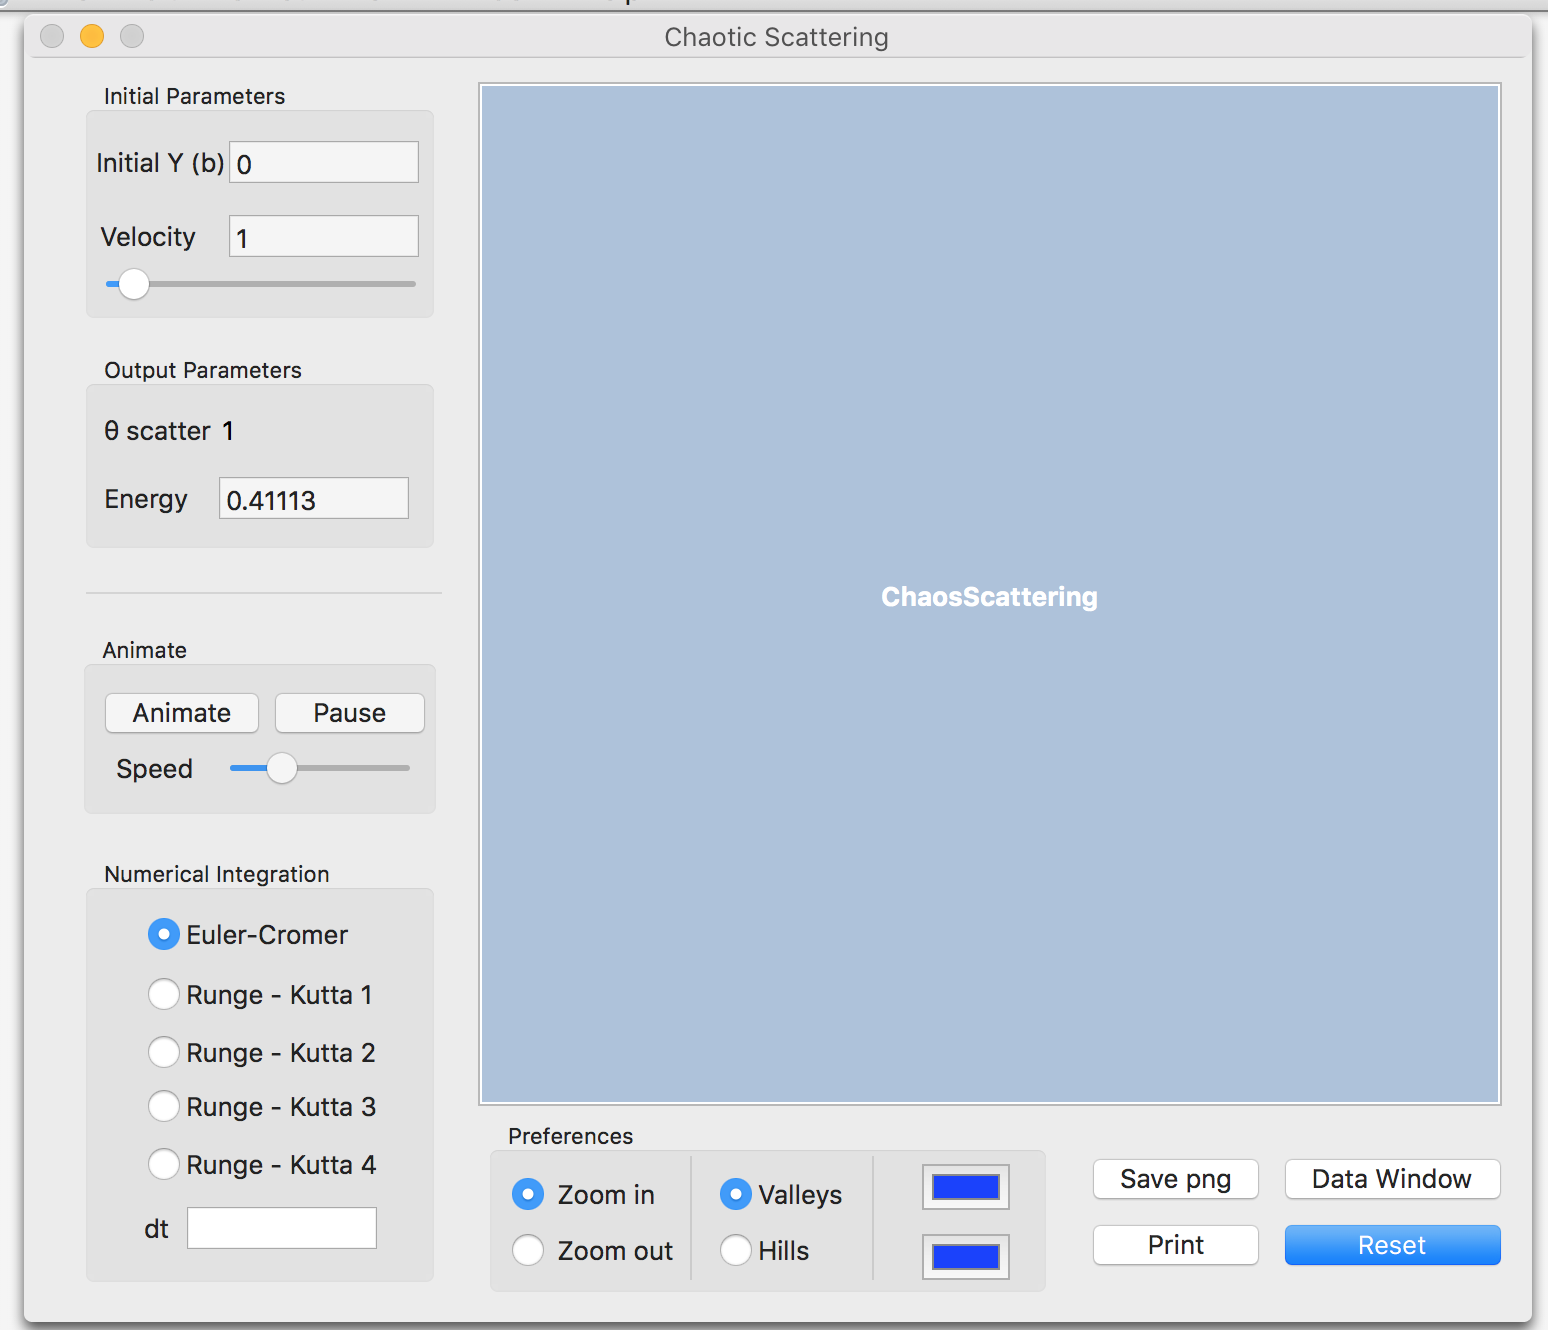
\includegraphics[width=0.7\textwidth]{ChaoticScatteringWindow.png}
	\caption
	[Screen Shot of the Interface]
	{A screen shot of the XML Interface.  }
	\label{fig:choasXML}
\end{figure}

\begin{figure}[h]
	\centering
	\includegraphics[width=0.7\textwidth]{About.png}
	\caption
	[Screen Shot of the About Box]
	{A screen shot of the About box for the application.  }
	\label{fig:about}
\end{figure}

Figure~\ref{fig:about} is that of the `About' box of the program, which contains the icon for the program, and text about the application. \\




Figure~\ref{fig:dataEntry} is that of the `Data Entry' box of the program, which appears when the user want to take data for an experiment. It is created when the user clicks the `Data Window' button.\\

\begin{figure}[h]
	\centering
	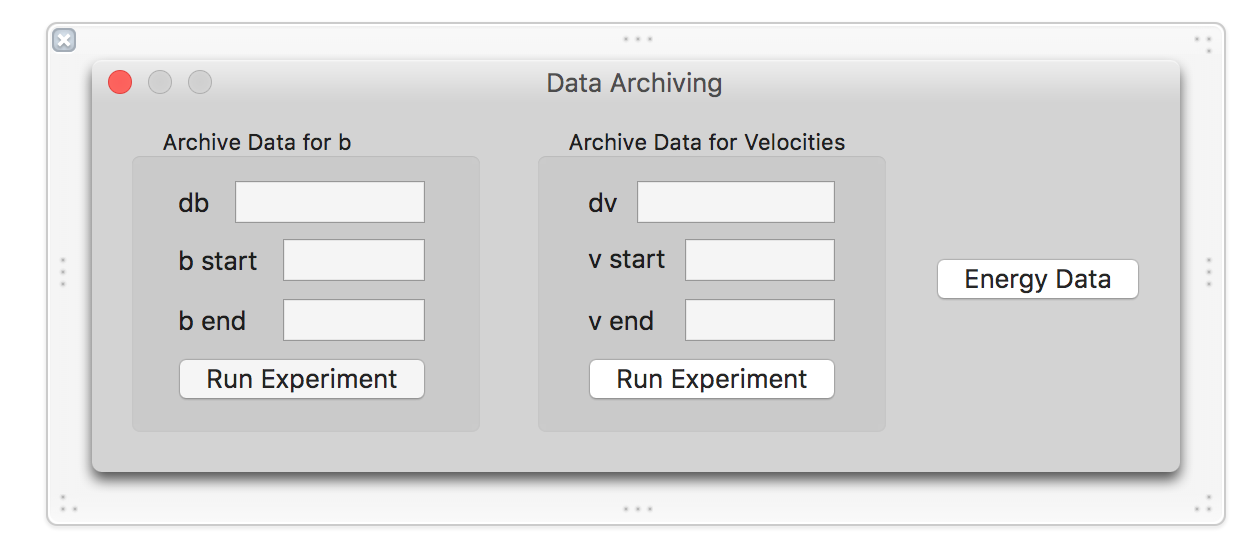
\includegraphics[width=0.7\textwidth]{dataEntry.png}
	\caption
	[Screen Shot of the Data Entry Window]
	{A screen shot of the data entry window of the program.  }
	\label{fig:dataEntry}
\end{figure}



%----------------------------------------------------------------------------------------
%	BIBLIOGRAPHY
%----------------------------------------------------------------------------------------


\nocite{*} 	%This command tells LaTeX to include ALL your BibTeX entries, even if you did not 
% \cite{} them, a practice which is strongly discouraged in mathematical papers. 
% We use it here because the listing of all the entries is the purpose of this assignment!


\bibliographystyle{plain}		% Using this bibliography style will ignore the annotations.

\bibliography{ChaosBib}		% This file should be replaced with the name of your .bib file.

\end{document}


\begin{thebibliography}{99}

%\bibitem{intro} This is a reference

\end{thebibliography}







\end{document}
